\documentclass[../../main.tex]{subfiles}
% \graphicspath{{\subfix{../images/}}}

\begin{document}
Como mencionamos anteriormente, las Redes Neuronales Convolucionales (RNCs) son un tipo
especializado de redes neuronales pensadas para el procesamiento de datos que tienen una
estructura de grilla \cite{deep-learning}. Ejemplos de estos datos son las series de
tiempo, que pueden pensarse como una grilla unidimensional y las imágenes, que pueden
verse como una grilla bidimiensional de píxeles.

Si bien las RNCs se han usado principalmente para el procesamiento de imágenes, en este
trabajo nos enfocaremos en su uso para analizar series de tiempo, en particular
unidimensionales. Veremos cómo su funcionamiento permite capturar patrones temporales en
los datos.

Sin entrar en detalles\footnotemark, una \textbf{serie de tiempo univariada o
unidimensional} se puede representar como un vector ordenado \(U\) de valores reales, en
el que cada valor corresponde a una medición en el tiempo sobre un determinado fenómeno:
\[
    U = (x_1, x_2, ..., x_N)
\]
donde \(N\) es la cantidad de observaciones.
\footnotetext{En una sección posterior, hablaremos más en profundidad sobre las
series de tiempo unidimensionales.}

Ahora bien, el término \textit{convolucionales} proviene del hecho que lo que caracteriza
a estas redes es la utilización de una operación matemática llamada
\textbf{convolución}\footnotemark \cite{deep-learning}. Las capas de la red que aplican
esta operación son llamadas \textit{capas convolucionales}. \footnotetext{En realidad, la
operación que está presente en estas redes es una relacionada con la convolución, llamada
\textbf{correlación cruzada}.}

La convolución toma dos argumentos: por un lado, la \textit{entrada} y por otro lado, un
\textit{filtro} o \textit{kernel}. En el contexto del ML, ambos son usualmente arreglos
multidimensionales de números reales, también comúnmente llamados tensores
\cite{deep-learning}. Intuitivamente, la operación consiste en ``deslizar'' el filtro
sobre la entrada, y en cada momento calcular el producto escalar. Para verlo más
claramente en el caso unidimensional, tomemos un ejemplo.

Dado como entrada a la convolución un vector \(\bm{x}\), si tomamos un filtro de
tamaño 3, dado por \(\bm{w}=(w_1, w_2, w_3)^T\), entonces el resultado de la convolución
es un vector \(\bm{z}\) en donde cada componente \(z_i\) es una suma pesada de las
entradas ``cercanas'':
\[z_i = w_1 x_{i-1} + w_2 x_{i} + w_3 x_{i+1}\]
\footnotetext[3]{Por conveniencia, el primer elemento de los vectores será indexado en 1,
y no en 0.}

En la Figura \ref{fig:conv1d-example}, se puede ver cómo se computan \(z_2\) y \(z_3\). Un
detalle a notar aquí es que al calcular \(z_2\) y \(z_3\), el filtro ``entra'' por
completo en la entrada, pero si quisiéramos calcular \(z_1\), pareciera que \(w_1\) no
tiene un valor de entrada con el cual multiplicarse. Existen alternativas para solucionar
este problema, que detallaremos más adelante.

\begin{figure}
    \centering
    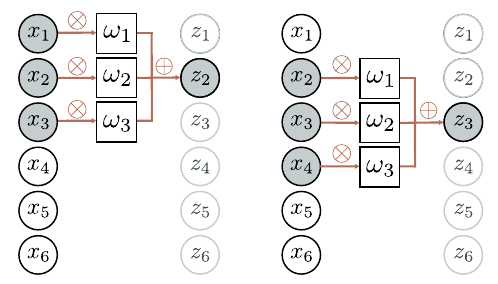
\includegraphics[width=0.65\textwidth]{figs/conv1d-example1.png}
    \caption{Fuente: \cite{prince2024understanding}. Ejemplo de convolución unidimensional
    con un filtro \(\bm{w}\) de tamaño 3.}
    \label{fig:conv1d-example}
\end{figure}

Si generalizamos y tomamos un vector \(\bm{x}\) de tamaño \(n\) correspondiente
a la entrada y un vector \(\bm{w}\) de tamaño \(l\) correspondiente al kernel,
entonces el resultado de la convolución es un vector \(\bm{z}\) donde:
\begin{equation}
    z_i = \sum_{j=1}^l w_j x_{j+i-(l+1)/2}
    \label{eq:convolution}
\end{equation}
En otras palabras, para generar cada componente \(i\) de la salida, se toma el producto
escalar entre el kernel \(\bm{w}\) y una parte de \(\bm{x}\) de largo \(l\) centrada en
\(x_i\) \cite{ai-a-modern-approach}.

La salida de la convolución suele llamarse \textbf{mapa de características}
(\textit{feature map}) \cite{deep-learning}, y resalta las áreas de la entrada que son
``similares'' a la característica que el filtro está tratando de capturar
\cite{hands-on-ML-sklearn-tf}. Para ver esto, tomemos otro ejemplo.

Supongamos que tenemos el filtro \(\bm{w} = (1, 0, -1)\) (de tamaño \(l=3\)). Entonces,
usando la Ecuación \ref{eq:convolution}, veamos qué calcula este filtro en cada
posición \(i\) de la salida:
\begin{align*}
    z_i =& \sum_{j=1}^3 w_j x_{j+i-(3+1)/2} \\
        =& \sum_{j=1}^3 w_j x_{j+i-2} \\
        =& w_1 x_{1+i-2} + w_2 x_{2+i-2} + w_3 x_{3+i-2} \\
        =& 1 \times x_{i-1} + 0 \times x_i + (-1) \times x_{i+1} \\
        =& x_{i-1} - x_{i+1}
\end{align*}
O sea, lo que hace es dada una posición \(i\) en la entrada, calcular la diferencia entre
el ``vecino'' izquierdo de \(i\) y el derecho. De esta forma, si para un \(i\) el valor
resultante de aplicar el filtro es positivo, quiere decir que hubo una transición de un
valor mayor a uno menor, y si es negativo, viceversa. En este caso, se podría decir que el
filtro ``detecta'' regiones de la entrada en donde hubo un cambio de tendencia.

Con esto, podemos ver que un filtro se encarga de identificar una característica
específica en la entrada, y que dicha característica depende de los valores del filtro.
Así, diferentes filtros actuando en conjunto podrán detectar diferentes características
puntuales.

Ahora que ya tenemos una intuición clara sobre qué hace una convolución, veamos
cómo esta operación se traslada a las redes neuronales. Para empezar, lo que va a
ocurrir ahora es que los parámetros a optimizar van a ser los pesos involucrados
en cada filtro.

Las redes convolucionales son un ejemplo de red Feedforward, ya que la información fluye
en una sola dirección. Ahora bien, vimos que en las redes totalmente conectadas, cada
neurona de una capa está conectada con todas las de la capa anterior. En cambio, en las
capas convolucionales lo que ocurre es que cada neurona está conectada con un subconjunto
de neuronas (consecutivas) de la capa anterior, sobre las cuales aplicará el filtro, y que
recibe el nombre de \textbf{campo receptivo}. Es importante notar que cada neurona de una
capa convolucional aplica el mismo filtro, por lo tanto todas ellas comparten los mismos
pesos. Esto significa que la cantidad de parámetros a aprender en una red convolucional es
menor que en una red totalmente conectada, y es algo que caracteriza a las RNCs. Este
comportamiento se puede ver en la Figura \ref{fig:fully-connected-vs-conv}.

\begin{figure}
    \centering
    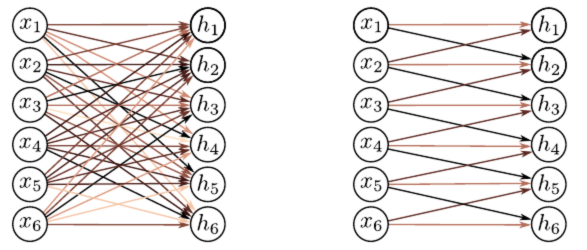
\includegraphics[width=0.7\textwidth]{figs/fully-connected-vs-conv.png}
    \caption{Fuente: \cite{prince2024understanding}. Capas de una red fully connected
    (izquierda) y capas convolucionales (derecha). Denotamos con \(x\) a la capa de la
    izquierda, y con \(h\) a la de la derecha, en ambos casos. En las capas de la fully
    connected, vemos que cada neurona de la capa \(x\) está conectada con todas las
    neuronas de la capa \(h\), habiendo un total de \(6 \times 6 = 36\) pesos entre ellas.
    En cambio, en la convolucional, asumiendo que se aplica un filtro de tamaño \(l=3\),
    tenemos que cada neurona de la capa \(h\) computa una suma pesada (con los mismos
    pesos) de \(l=3\) neuronas consecutivas de la capa \(x\).}
    \label{fig:fully-connected-vs-conv}
\end{figure}

Con esta idea de campo receptivo, podemos pensar en una red con dos capas convolucionales
seguidas y en las que se aplica un filtro de tamaño 3. Lo que va a ocurrir entonces es que
las neuronas de la primera capa oculta toman una suma pesada de conjuntos de 3 neuronas
consecutivas de la capa de entrada. Luego, las unidades de la segunda capa oculta toman
una suma pesada de conjuntos de 3 neuronas consecutivas de la primera capa oculta, que son
a su vez sumas pesadas de 3 neuronas de entrada. Por lo tanto, las neuronas de la segunda
capa oculta en realidad tienen un campo receptivo de 5 neuronas. De esta forma, el campo
receptivo de las unidades en las capas siguientes va aumentando \cite{prince2024understanding}.
Esto provoca que la primera capa oculta se concentre en características de bajo nivel,
más específicas, luego la siguiente en otras de mayor nivel como resultado de integrar
las anteriores, y así sucesivamente \cite{hands-on-ML-sklearn-tf}.

Hasta ahora vimos una capa convolucional que aplica solamente un filtro, lo que nos va a
dar como resultado solamente un mapa de características. Sin embargo, una misma capa puede
aplicar varios filtros (todos del mismo tamaño), cada uno de los cuales va a generar su
propio feature map. Para esto, lo que se hace es darle a la capa una ``profundidad'' de
tantos filtros como querramos aplicar sobre la entrada, obteniendo de esta forma un feature
map para cada nivel profundidad, cada uno capturando una característica puntual de la imagen.
Así, se suele decir que una capa tiene varios \textit{canales}.

Algo que cabe notar en este punto es que cuando una neurona aplica el filtro
correspondiente sobre las de la capa anterior, si esta última tiene varios canales,
entonces el filtro es aplicado en todos ellos. Es decir, si por ejemplo la capa anterior
tenía \(C\) canales y el filtro tiene tamaño \(l\), entonces al aplicar el filtro, ahora
vamos a tener una cantidad de pesos \(l \times C\). Esto se puede ver en la Figura
\ref{fig:conv-layer-multi-channel}.

\begin{figure}
    \centering
    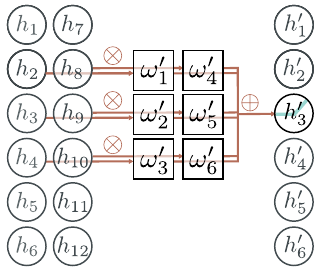
\includegraphics[width=0.4\textwidth]{figs/conv-layer-multi-channel.png}
    \caption{Fuente: \cite{prince2024understanding}. La capa de neuronas \(h_i\) tiene
    dos canales: aquel formado por las neuronas \(h_1\) a \(h_6\) y aquel formado
    por las neuronas \(h_7\) a \(h_{12}\). La capa de neuronas \(h'_i\) aplica un
    filtro de tamaño \(l=3\) sobre cada uno de los canales de la capa anterior. Por
    lo tanto ahora termina habiendo \(2 \times 3 = 6\) pesos entre cada neurona de la
    capa \(h'_i\) y la capa \(h_i\).}
    \label{fig:conv-layer-multi-channel}
\end{figure}

Además de la cantidad de filtros en una capa, y su tamaño \(l\), existen otros
hiperparámetros de las capas convolucionales: \vspace{-0.25cm}
\begin{itemize}[noitemsep]
    \item El \textbf{paso} (\textit{stride}), que representa la distancia entre dos campos receptivos
    consecutivos. Un stride igual a 1 quiere decir que el filtro se aplica en cada
    posición de la entrda.
    \item El \textbf{relleno} (\textit{padding}), que controla cuántos valores
    ``fantasma'' se agregan artificialmente a los extremos de la entrada de forma tal que
    el tamaño de la salida de la convolución no sea tanto menor al de la entrada. En la
    práctica, se usa el 0 para este relleno (\textit{zero-padding}). Con esto, se
    puede computar el valor de \(z_1\) que presentamos como ejemplo anteriormente.
    \item La \textbf{dilatación} (\textit{dilation}), que determina cuántos 0s se
    intercalan en los pesos del filtro. Con este parámetro, se puede convertir un filtro
    de \(l=5\) a uno ``dilatado'' de tamaño 3 fijando el segundo y cuarto elementos en 0.
    Esto permite seguir ``integrando'' la información de una región de la entrada de
    tamaño 5 pero requiriendo solamente 3 pesos para hacerlo
    \cite{prince2024understanding}.
\end{itemize}

Otros de los componentes particulares de las RNCs son las capas de \textit{pooling}, cuyo
objetivo principal es reducir el tamaño del mapa producido por la convolución
\cite{hands-on-ML-sklearn-tf}. Es decir, se aplican luego de la convolución y lo que hacen
es reemplazar valores contiguos presentes en una determinada sección del mapa por una medida
resumen de ellos, entre las cuales algunas comúnmente utilizadas son el máximo
(\textit{max pooling}) y el promedio (\textit{average pooling}). Esta reducción de tamaño
no solo disminuye la cantidad de parámetros sino que también hace a la red más robusta
ante desplazamientos de la imagen \cite{hands-on-ML-sklearn-tf}.

Una capa convolucional típica de una RNC se compone de tres etapas: en primer lugar, se
producen las convoluciones, que se encargan de producir activaciones lineales; luego, cada
una de estas activaciones pasa por una función de activación no lineal; y finalmente se
aplica pooling para reducir el tamaño de la salida \cite{deep-learning}. Y así, una RNC
profunda se compone de varias de estas capas.

\bigskip
Ahora bien, en este trabajo nosotros utilizaremos este tipo de redes para resolver la
tarea de \textbf{clasificación de series de tiempo}. Esto es: dada una serie de tiempo
como entrada de la red, que esta sea capaz de predecir a qué categoría corresponde. Para
ello, lo que se suele hacer en estas redes es agregar, luego de la última capa
convolucional, una capa de \textbf{aplanado} (\textit{flatten}), la cual no posee pesos
aprendibles y simplemente convierte el tensor resultante de la capa anterior en uno
unidimensional. Por ejemplo, si esta consiste de \(k\) feature maps de longitud \(n\) cada
uno, entonces la capa de flatten dará como resultado un vector unidimensional de tamaño
\(kn\).

El paso anterior es necesario ya que las capas siguientes que se agregan para hacer la
clasificación son totalmente conectadas que, como vimos anteriormente, aceptan únicamente
entradas unidimensionales. Entonces, lo que ocurre es que el vector de tamaño \(kn\) es
procesado por las diferentes capas densas hasta llegar a la de salida.

En problemas de clasificación con más de dos categorías, esta última capa suele tener
tantas neuronas como clases haya. En cambio, para tareas de clasificación binaria, como en
nuestro caso, se utiliza habitualmente una única neurona con una función de activación
sigmoide, cuya salida representa la probabilidad de que la secuencia de entrada pertenezca
a la clase positiva (aquella asociada con la etiqueta 1).

\end{document}